\documentclass[a4paper]{report}
\author{Jure Kos}
\title{Vaja 69, Absorpcija sevanja gama}
\date{22.4.2022}
\usepackage{graphicx}
\graphicspath{ {./images/} }

\begin{document}

\maketitle

\chapter*{Uvod}
Pri radioaktivnem razpadu večina atomskih jeder oddaja tudi sevanje gama, to je
kratkovalovno rentgensko svetlobo. Valovna dolžina sevanja gama, ki ga sevajo
radioaktivne snovi, je od okoli 1 nm do $10^{-3}$ nm, kar ustreza energiji fotonov od nekaj keV do nekaj MeV. Če vzporeden curek sevanja gama s pretokom delcev $\phi_0$vpada pravokotno na zaslon z debelino d, se na drugi strani zaslona tok zmanjša. S povečevanjem debeline zaslona, dobimo odvisnosti pretoka delcev $\phi$ od debeline zaslona, kot kaže slika:\\
Vidimo, da pretok pojema eksponentno z debelino plasti. Debelino, pri kateri pade
tok sevanja gama na polovico prvotne vrednosti, imenujemo razpolovna debelina. Če
debelino zaslona poveČamo za razpolovno debelino, se pretok zmanjša za polovico.
Tako velja:

\[\phi = \phi_0e^{-\mu d}\]

kjer je $\phi_0$ pretok v vpadnem curku, d je debelina zaslona, $\mu$ pa je koeficient absorpcije. Ta je značilen za snov in je odvisen tudi od energije sevanja gama. Med pripravami za zaznavanje sevanja gama je najbolj znan Geiger-Müllerjev števec(GM). Števec sestavlja kovinska cev kot zunanja elektroda in soosno (koaksialno) nameščena tanka žička kot druga elektroda. Cev je zaprta in napolnjena z mešanicoplinov pri tlaku okoli 100mbar.\\
Števec je priključen na enosmerno napetost tako, da je žička v sredini pozitivna.
Ioni in elektroni, ki jih pri preletu skozi plin ustvari delec gama, sprožijo v cevi kratkotrajen električni tok. Tokovni sunek zaznamo z elektronsko števno napravo. Upoštevati je treba, da le vsak stoti foton sevanja gama pri preletu sproži tak sunek. Razpadanje radioaktivnih atomskih jeder je slučajni pojav, zato pri večkratnih merjenjih v enakih okoliščinah ne naštejemo natančno enakega števila sunkov. Poissonova porazdelitev

\[W_N = \frac{\overline{N}^N}{N!}e^{-\overline{N}}\]

opisuje njihovo raztresenost okoli povprečne vrednosti $\overline{N}$, ki jo izračunamo po znanem splošnem predpisu. Izkaže se, da je pri tej porazdelitvi efektivni odmik od povprečja $\sigma = \sqrt{\overline{N}}$
Relativno število razpadov v časovnem intervalu dt določa verjetnost razpada $\lambda$ kot:

\[\frac{dN}{N}=-\lambda	dt\]

Odtod sledi tudi formula za upadanješstevila nerazpadlih jeder po eksponentnem
zakonu z razpolovnim časom $T_{\frac{1}{2}}=\frac{ln2}{\lambda}$.

\chapter*{Naloga}

1. Preizkusi enačbo $\sigma = \sqrt{\overline{N}}$ z večkratnim štetjem razpadov v enakih časovnih
intervalih.\\
2. Izmeri razpolovno debelino svinca za sevanje gama, ki jih pri radioaktivnem
razpadu seva kobaltov izvor!\\
3. Določi porazdelitev časovnih intervalov med zaporednimi razpadi.

\section*{Potrebščine}
1. Vernierjev detektor - GM števec,\\
2. vmesnik,\\
3. radioaktivni preparat,\\
4. svinčene ploščice.

\chapter*{Meritve}
\[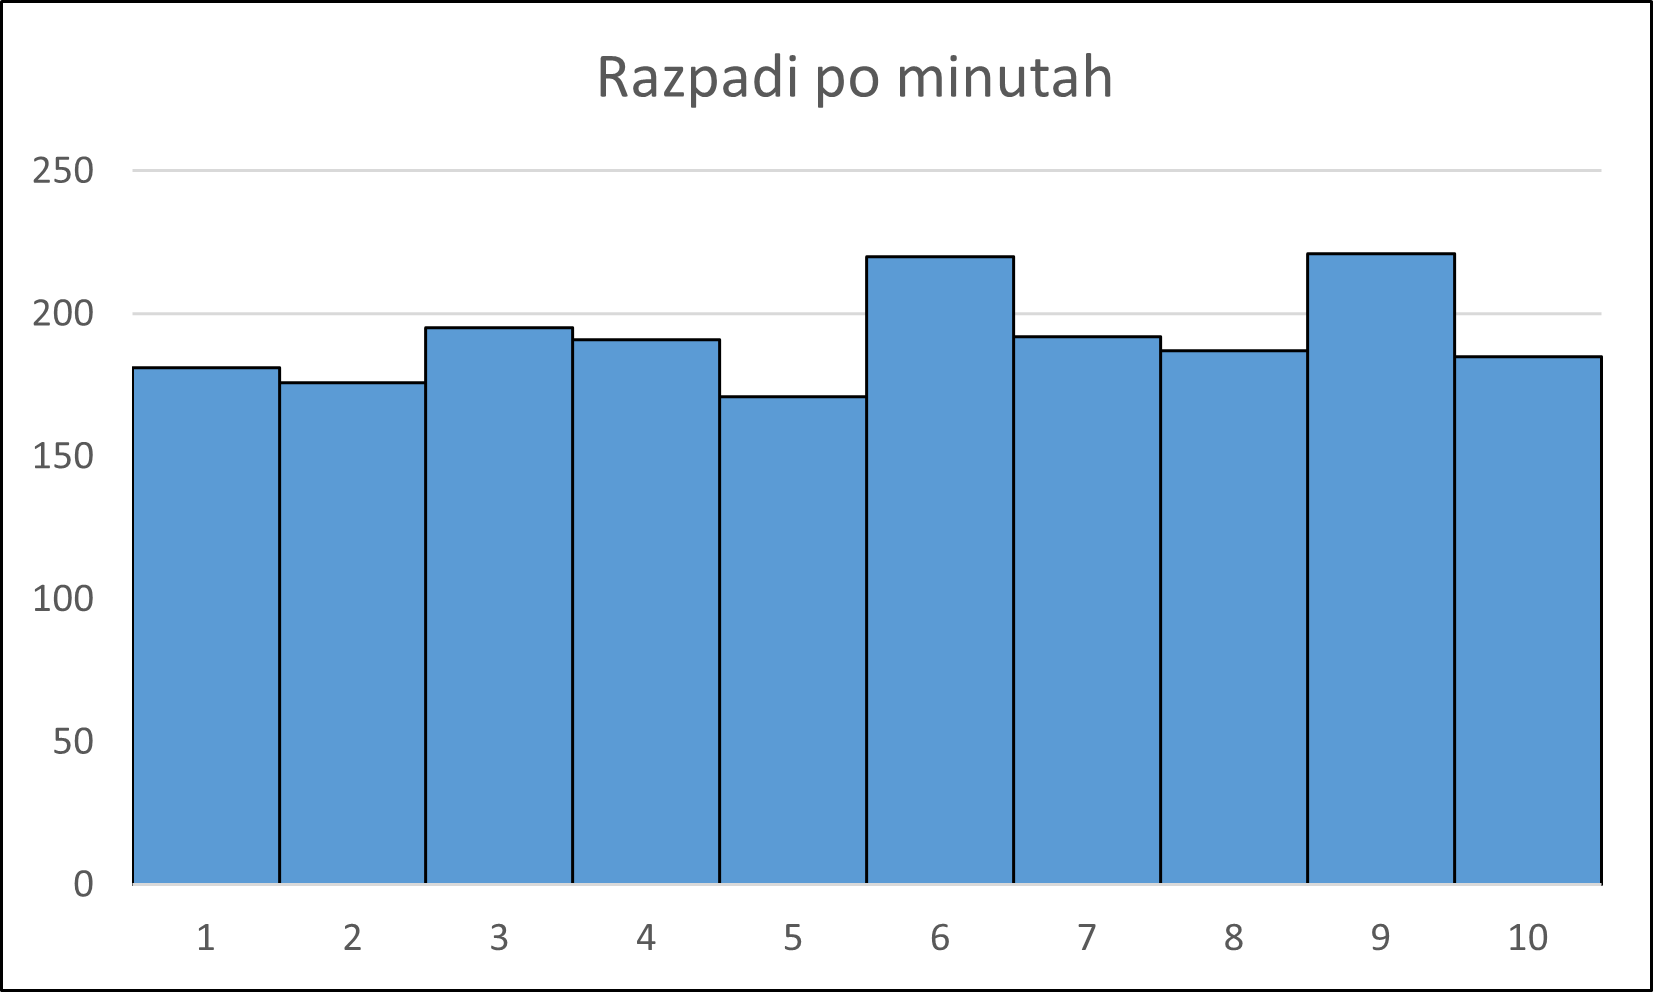
\includegraphics[width=\textwidth]{Minute.png}\]
Iz histograma razberemo $\overline{N}=192$ in povprečni efektivni odmik $\sigma = 12$ in lahko preverimo točnost enačbe $\sigma = \sqrt{\overline{N}}=13,9$ in dobimo podobno vrednost. Iz tega sledi, da je enačba točna ampak bi bil rezultat boljši, če bi merili dlje časa.

\newpage

\[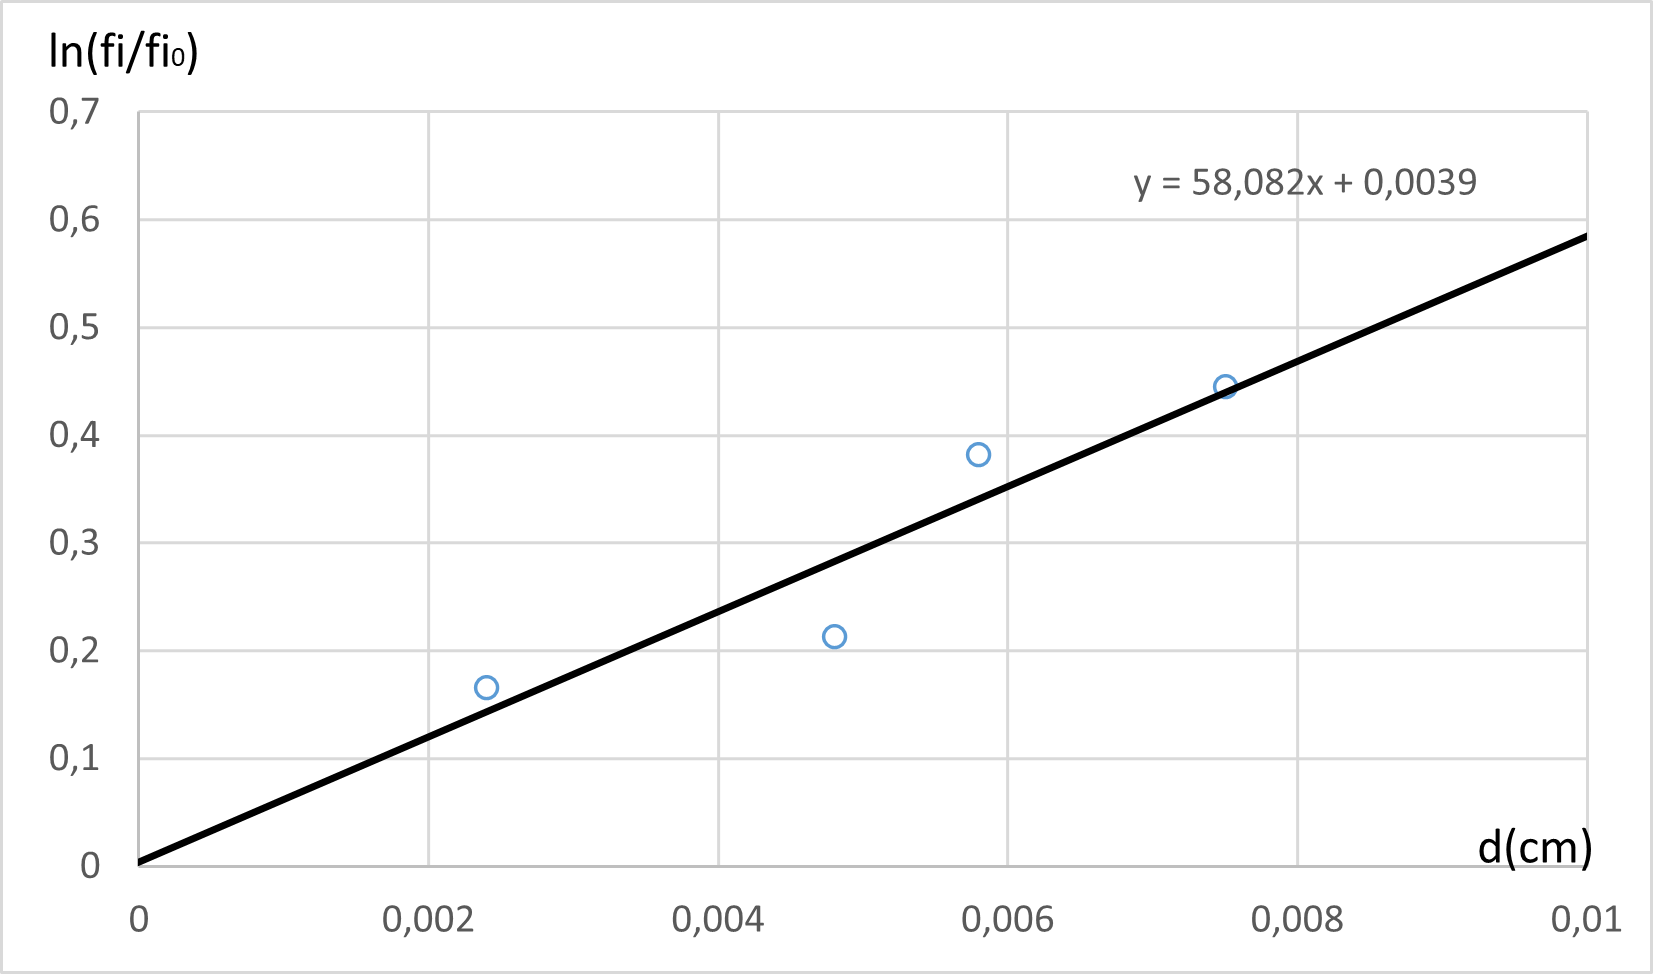
\includegraphics[width=\textwidth]{Konstanta.png}\]
Iz grafa lahko razberemo $\mu = 0,44/cm$ Iz tega lahko izračunamo razpolovno debelino $d=-ln(\phi/\phi_0)/\mu=0,52/cm$. Dejanska vrednost pa je 0,59, kar kaže na natančnost meritev.
\chapter*{Grafi}
Graf števila intervalov med razpadi.
	\[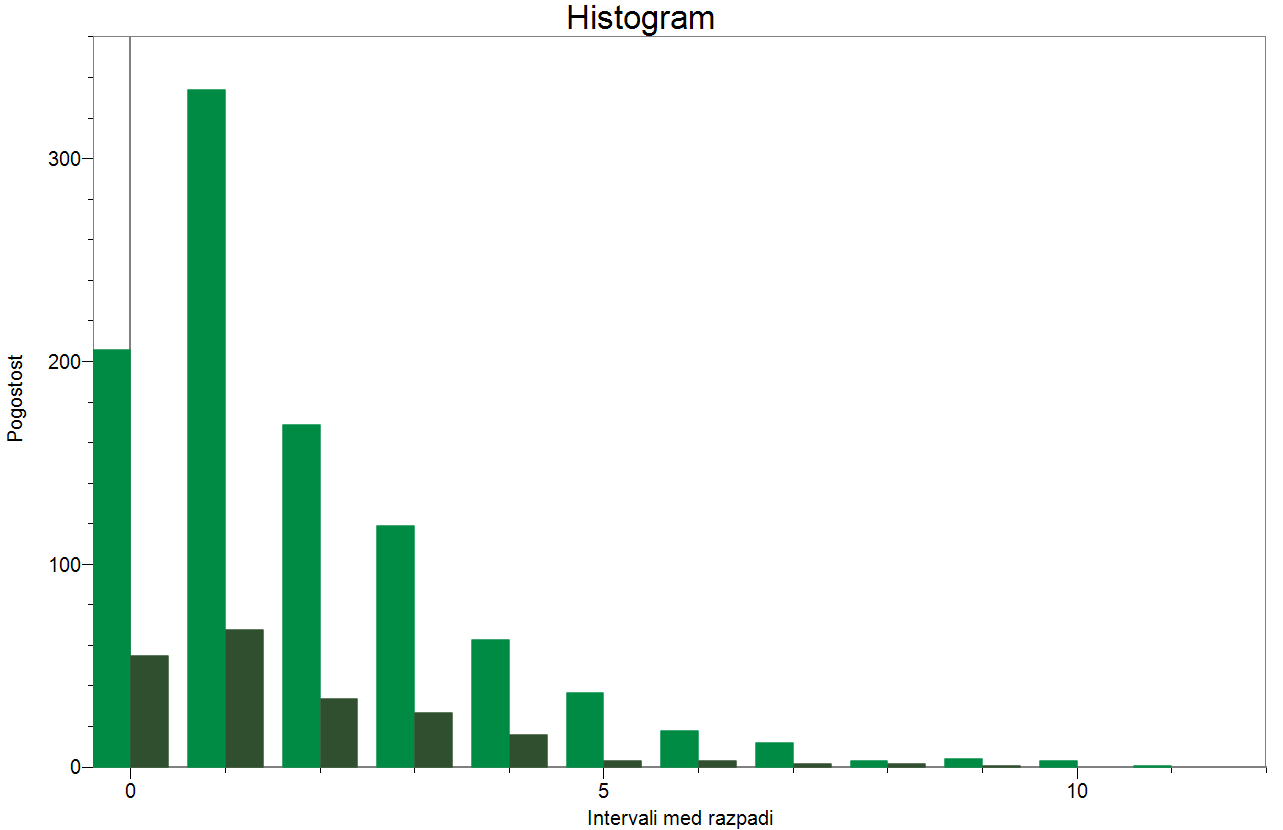
\includegraphics[width=\textwidth]{Histogram.png}\]

\end{document}